% =======================================================================================
\section{Related Work}
\label{app:related}
% =======================================================================================

\ac{lisa} will resolve thousands of \acp{gb}, and within a narrow frequency band
several of them overlap. Two routes lead to their posteriors. The global fit samples all
resolvable sources with the likelihood: it is the reference for what the data support, but it
is run again for every new stretch of data. Amortised estimators learn the posterior once and
then draw from it in seconds, but so far for one source, two ordered ones in a narrow band, or a
factorised set of toy signals. This work is the amortised route at the global fit's unit of
work: the joint posterior of the $S$ sources of a frequency window, $S$ from
\ResultsNarrowCounts{} on the narrow band to \ResultsFullCounts{} on the full band, $8S$ parameters with
the full instrument response, for windows anywhere in
\qtyrange{\RelatedWorkFzeroLow}{\RelatedWorkFzeroHigh}{\milli\hertz}, drawn by conditional flow matching from the
prior with no likelihood evaluation. \Cref{tab:related-closest} places it among the \ac{gb}
methods; the paragraphs below cover the wider literature it draws on.

\begin{table}[!htbp]
\caption{Inference of galactic binaries, as each work reports it. \emph{Joint}: one posterior
over overlapping sources, not a product over them. \emph{Likelihood}: evaluated to draw a
posterior sample.}
\label{tab:related-closest}
\centering
\small
\setlength{\tabcolsep}{4pt}
\renewcommand{\arraystretch}{1.15}
\newcolumntype{L}[1]{>{\raggedright\arraybackslash}p{#1}}
\newcolumntype{C}{>{\centering\arraybackslash}p{1.25cm}}
\newcommand{\rwyes}{$\checkmark$}
\newcommand{\rwno}{\textcolor{gray}{--}}
\newcommand{\rwgroup}[1]{\multicolumn{7}{@{}l}{\textsc{#1}}\\[1pt]}
\begin{tabular}{@{}L{2.9cm}L{2.8cm}CCCL{3.9cm}L{1.8cm}@{}}
\toprule
work & sources per posterior & joint & amortised & likelihood & signal, data and prior & reference \\
\midrule
\rwgroup{likelihood-based}
\acs*{rjmcmc} global fit \citep{littenberg2020global,katz2024efficient,strub2024global}
  & all resolvable ones, their number inferred
  & \rwyes & \rwno & \rwyes
  & full response; the whole band, segment by segment, with the noise and other source classes
  & \rwno \\
flows as priors and proposals \citep{korsakova2024neural,sasli2026learned}
  & 1 per flow, fitted to chains; proposed for the global fit
  & \rwno & \rwno & \rwyes
  & inside the global fit's sampler
  & its chains \\
\midrule
\rwgroup{amortised}
\citet{delmond2026neural}, \acs*{nsf}
  & 1; 2 as a proof of concept, ordered by $f_0$
  & 2 only & \rwyes & \rwno
  & full response; $A$, $E$; $\Tobs=\qty{1}{\year}$; $f_0$ within $\pm\qty{2}{\micro\hertz}$ of a fixed centre; \acs*{snr} \numrange{10}{100}
  & \acs*{mcmc}; P--P \\
\citet{mao2025robust}, \acs*{fmpe}
  & 1, with 3 free parameters
  & \rwno & \rwyes & \rwno
  & \acs*{gb}-like; \acs*{tdi} channel $A$ only; \qtyrange{30}{90}{\day} with gaps; narrow boxes around the truth
  & \acs*{maf} \\
SlotFlow \citep{houba2025slotflow}, \acs*{nsf} per slot
  & up to 10, their number inferred; slots matched to injections
  & factorised & \rwyes & \rwno
  & sinusoids in white noise, no response
  & \acs*{rjmcmc} \\
\midrule
this work, flow matching
  & 2 to 16, fixed per run, ordered in $f_0$
  & \rwyes & \rwyes & \rwno
  & full response; $A$, $E$, $T$; $\Tobs=\qty{\RelatedWorkTobs}{\year}$; $(f_0, \fdot, \Amp)$ from a
    Galactic catalogue over \qtyrange{\RelatedWorkFzeroLow}{\RelatedWorkFzeroHigh}{\milli\hertz}; most sources
    below the noise, visible ones at \acs*{snr} \numrange{\RelatedWorkSnrLow}{\RelatedWorkSnrHigh}
  & joint \acs*{mcmc}; Fisher \\
\bottomrule
\end{tabular}
\end{table}

\paragraph{Likelihood-based inference of galactic binaries.}
The \ac{lisa} global fit samples all resolvable sources with reversible-jump
\citep{green1995reversible}, parallel-tempered \citep{earl2005parallel} \ac{mcmc}, segment by segment
for the \acp{gb} and jointly with the other source classes and the noise
\citep{littenberg2020global,littenberg2023prototype,katz2024efficient,strub2024global,deng2025modular};
sequential Monte Carlo parallelises its trans-dimensional moves \citep{demasi2026massively}.
Neural density estimators enter it as fitted priors, proposals and compact catalogues
\citep{korsakova2024neural}, each flow fitted to one source's chains, and as learned birth proposals,
which \citet{sasli2026learned} show on non-\acs{gb} benchmarks to help once the fit has equilibrated
rather than while it is assembled. Fisher forecasts
\citep{cutler1998angular} give local Gaussian widths, reliable only at high \ac{snr}
\citep{vallisneri2008use}. We use both only as references (\cref{app:evaluation,app:mcmc}): a
joint \ac{mcmc} over all \McmcJointDim{} parameters of each eval injection, and Fisher widths at
the injection. An amortised window posterior could in turn serve a global fit as a
proposal or as the initial state of its chains.

\begin{figure}[t]
\centering
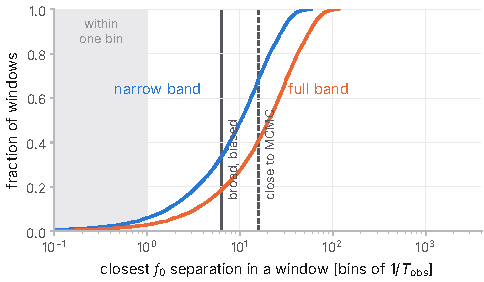
\includegraphics[width=3.25in]{figures/crowding.pdf}
\caption{How crowded the training windows are: the distribution of the closest $f_0$ separation
among the \RelatedWorkSourcesWord{} sources of a window, over \RelatedWorkCrowdingWindows{}
training windows per band (\cref{eq:priors-window}), in each analysis's own bins of $1/\Tobs$
(\qty{\RelatedWorkDelmondTobs}{\year} for \citet{delmond2026neural}, \qty{\RelatedWorkTobs}{\year} here). Vertical lines: the two source pairs of
\citet{delmond2026neural}, \RelatedWorkDelmondEasiest{} bins apart (close to \ac{mcmc}) and
\RelatedWorkDelmondHardest{} (broad, sometimes biased). In the narrow band \qty{\RelatedWorkCloserNarrow}{\percent} of
windows hold a pair closer than their hardest one, in the full band \qty{\RelatedWorkCloserFull}{\percent}.}
\label{fig:related-crowding}
\end{figure}

\paragraph{Amortised posteriors for galactic binaries.}
\citet{delmond2026neural} train a neural spline flow on the frequency-domain $A$ and $E$ data
of a narrow band. For one source their posteriors match an \ac{mcmc} at \qty{1}{\milli\hertz}, come out slightly
wider at \qty{5}{\milli\hertz} and clearly wider in $f_0$ and sky at \qtyrange{10}{15}{\milli\hertz} and over a \qty{0.5}{\milli\hertz} band. For two sources they impose
$f_{0,1}\le f_{0,2}$, since an unordered flow put one mode on each labelling; their pair
\RelatedWorkDelmondEasiest{} bins apart is close to \ac{mcmc}, the pair \RelatedWorkDelmondHardest{}
bins apart broad and sometimes biased. \citet{mao2025robust} apply \ac{fmpe} to gapped data of one
source with three free parameters. SlotFlow \citep{houba2025slotflow} infers the number of
components with a classifier and gives each a slot of a shared flow trained with Hungarian
matching; its posterior factorises over the slots given a shared context, which cannot carry
correlations between close sources, and on sinusoid mixtures its frequency widths are two to
three times those of \ac{rjmcmc}. Population properties of the \acp{gb} can be inferred without any
per-source posterior \citep{srinivasan2025simulation,desanti2026inferring}. SlotFlow was presented
as a step towards \ac{lisa} at the AI for Gravitational Waves workshop (CERN, May 2026), where the
\ac{lisa} global fit was also discussed as a target for scalable simulation-based inference; none of
the amortised \ac{gb} works above has, to our knowledge, been extended to a joint posterior over more
than two sources under the \ac{lisa} response.

Our sources are not placed by hand but drawn from the prior, and \cref{fig:related-crowding}
shows what that implies. In the narrow band the closest two sources of a window are a median
\RelatedWorkClosestNarrow{} bins apart, closer than Delmond et al.'s hardest pair in
\qty{\RelatedWorkCloserNarrow}{\percent} of windows and within one bin in \qty{\RelatedWorkSubBinNarrow}{\percent}; in the
full band, whose windows are wider, the median is \RelatedWorkClosestFull{} bins and only
\qty{\RelatedWorkCloserFull}{\percent} of windows are that crowded. Among the Galaxy's resolvable
sources overlap is rarer: fewer than \qty{1}{\percent} of pairs above \ac{snr} 7 have a match above
one half after a year \citep{littenberg2020global}.
\textcolor{red}{TODO(analysis): width ratio to the joint \ac{mcmc} against closest-pair separation,
for the runs of \cref{app:results}.}

\paragraph{Neural posterior estimation for gravitational waves.}
Amortised posteriors are established for ground-based detectors
\citep{chua2020learning,green2020gravitational,green2021complete,gabbard2022bayesian,dax2021real,dax2025real},
with importance sampling to the exact posterior \citep{dax2023neural}, equivariance under
detector time shifts \citep{dax2022group}, flow matching \citep{dax2023flow} and transformers
\citep{kofler2026flexible}; ground-based overlapping signals have been analysed jointly
\citep{langendorff2023normalizing,alvey2023crowded,bhardwaj2023sequential,hu2025hierarchical,zhao2025compact}.
For \ac{lisa}, normalising flows \citep{du2024advancing,spadaro2026accurate}, flow matching
\citep{liang2024rapid}, sequential neural likelihoods \citep{martinvilchez2025efficient} and
flow-guided tempering \citep{liang2026fluxmc} treat massive black-hole binaries; truncated
ratio estimation treats extreme mass-ratio inspirals \citep{cole2026sequential} and stochastic
backgrounds \citep{alvey2024simulation,alvey2025leveraging}. Deep networks also detect and
separate overlapping \ac{lisa} signals, without posteriors
\citep{zhao2023space,houba2025deep,ma2026deep}; \citet{niu2026extracting} review the overlap
problem, and \citet{cuoco2025applications} and \citet{zhao2025dawning} machine learning for
gravitational waves.

\paragraph{The phase.}
A recurring failure of these estimators is the initial or coalescence phase, whose posterior
the network often leaves at the prior \citep{dax2023neural,du2024advancing,cole2026sequential}.
DINGO and Dingo-T1 therefore draw it outside the network, from the likelihood
\citep{dax2023neural,kofler2026flexible}, which we exclude. For a \ac{gb} the signal is linear in
four amplitudes \citep{jaranowski1998data}, and the two circular polarisations carry the
phases $\phi_0\pm2\psi$ \citep{whelan2014new}. Our chart (\cref{eq:chart}) uses these helicity
amplitudes as flat complex coordinates: the four $(\psi,\phi_0)$ copies of a source
(\cref{eq:psi-phi-symmetry}) fold into one point, and each phase becomes the angle of a
coordinate whose radius sets how well it is known (\cref{app:chart}). \citet{delmond2026neural}
found broader posteriors when their flow predicted the four linear amplitudes directly; ours
differ from those by the rotation into helicities and an $\operatorname{asinh}$ warp of the
radius in \ac{snr} units.

\paragraph{Flow matching and diffusion for posterior estimation.}
Flow matching \citep{lipman2023flow,liu2023flow,albergo2023building} entered simulation-based
inference as \ac{fmpe} \citep{dax2023flow}, where it matches or beats normalising flows for massive
black-hole binaries \citep{liang2024rapid} and exoplanet atmospheres \citep{gebhard2025flow};
\citet{arruda2025diffusion} review diffusion and flow models for simulation-based inference.
Score-based alternatives amortise over arbitrary conditionals \citep{gloeckler2024allinone} or
compose per-observation scores \citep{geffner2023compositional,sharrock2024sequential}. Our
objective departs from standard \ac{fmpe} in two ways, argued in \cref{app:fm}: the Gaussian base
is placed and scaled per source by a frame the network reads off the data and trains on the
likelihood of the true sources, so the flow sees order-one widths at every \ac{snr}; and the
network predicts a Gaussian over the endpoint, trained on its likelihood, and samples with the
velocity its mean implies, as FrameFlow does with a point estimate \citep{yim2023fast}. The learned width
weights each point's error by its own irreducible part, as learned task uncertainties weight tasks
\citep{kendall2018multi}, in place of fixed weights over time
\citep{karras2022elucidating,kingma2023understanding}.

\paragraph{Label switching.}
A posterior over exchangeable sources has one mode per labelling. \ac{mcmc} removes them by
relabelling or by an ordering constraint \citep{stephens2000dealing,jasra2005markov}; for \ac{lisa},
\citet{buscicchio2019label} and the global fit \citep{littenberg2020global} order \acp{gb} by
frequency, and amortised mixture models face the same problem \citep{kucharsky2026amortized}.
Neural estimators order the sources \citep{delmond2026neural}, match slots to injections in
the loss \citep{houba2025slotflow}, or make the model permutation-equivariant
\citep{zaheer2017deep,lee2019set,klein2023equivariant} and align base and target by
optimal-transport couplings over permutations \citep{tong2024improving,klein2023equivariant}.
We order by frequency, as the global fit does (\cref{app:chart-slots}): each slot then has a
frame of its own, which an equivariant model, whose slots are interchangeable, could not give.
The ordering has a boundary between sources close in frequency, the overlap that is hardest to
resolve, where the ordered posterior is folded and the flow must place the edge. The evaluation,
which compares draws with injections, pairs them by matching (\cref{app:evaluation}).

\paragraph{Transformers for simulation-based inference.}
Dingo-T1 \citep{kofler2026flexible} feeds the strain as tokens of 16 frequency bins; the
Simformer \citep{gloeckler2024allinone} is a transformer over parameters and data alike; t-\ac{fmpe}
\citep{vandermeulen2026fast} uses one to generate a variable number of components. Our network
(\cref{app:network}) is a multimodal diffusion transformer
\citep{peebles2023scalable,esser2024scaling} with the sources as one stream of tokens and the
data as another, short-time Fourier tokens of \RelatedWorkPatch{} bins on a frequency axis
shared through rotary embeddings \citep{su2024roformer}. Its attention is one-way: the data
never attend to the sources, so the data stream is encoded once per observation and reused for
every posterior draw in training and every step of the sampler. Frame registers and attention sinks
\citep{xiao2024efficient,darcet2024vision} and a Muon optimiser \citep{jordan2024muon,liu2025muon}
with a warmup--stable--decay schedule \citep{hu2024minicpm,hagele2024scaling} (\cref{app:training})
complete it.

\subsection*{Recent Work, 2025--2026}
\label{app:related-recent}
% From the 2026-11-09 survey (DINGO line, the Korsakova group and LISA machine learning, and the
% AI for Gravitational Waves workshop at CERN, indico 1640502). Each claim below follows the
% paper's abstract as the survey read it; check before moving any of it to the main text.

\paragraph{The DINGO line.}
Since flow matching \citep{dax2023flow} and Dingo-T1 \citep{kofler2026flexible}, the DINGO authors
have amortised over whole catalogues: Dingo-Pop \citep{leyde2026end} embeds each event as a token
and a transformer returns the population posterior from 25 to 1000 events, the closest DINGO
precedent for a transformer over a variable set of inputs, though its output is a posterior over
hyperparameters, not a joint posterior over the sources. Earlier work adapted the network to
shifts of the noise distribution \citep{wildberger2023adapting}, which our fixed-\ac{psd} simulator
does not need yet (\cref{app:forward-model-limits}); DINGO-IS reaches next-generation ground-based
networks \citep{santoliquido2025fast}, and DINGO for \ac{lisa}'s massive black-hole binaries
\citep{spadaro2026accurate} remains its only space-based application. \citet{dax2026introduction}
give a tutorial on Bayesian and frequentist simulation-based inference with machine learning.

\paragraph{Amortised inference becomes tooling.}
On ground-based data, neural posterior estimation now runs in production alerts
\citep{marx2026likelihood} and in user-facing packages \citep{pinchbeck2026bilbyflow}; labrador
\citep{roulet2026domain} heterodynes the data against a reference waveform and folds the parameter
space to remove multimodality, close in spirit to our frame and our folded phases, though its
reference comes from a per-event optimisation and our frame from the network. \citet{kolmus2024tuning}
find that the accuracy of neural posterior estimation follows how densely the training prior covers
each region, which bears on our catalogue prior, where loud sources are rare
(\cref{app:priors}). Likelihood-based samplers on GPUs are closing the gap for single sources: a
GPU nested sampler returns binary-neutron-star posteriors from the prior in minutes
\citep{yallup2026abinitio}. For one source, speed alone is a weakening argument for amortisation;
the joint posterior of many overlapping sources, whose chains take hours
(\cref{app:mcmc-cost}), is where it still pays.

\paragraph{Flow matching, diffusion and consistency models.}
Outside the DINGO authors' work, flow matching for gravitational-wave posteriors appears for single
sources only: intermediate-mass black-hole binaries \citep{raymond2025simulation}, pulsar-timing
backgrounds \citep{liang2026accelerating}, and extreme mass-ratio inspirals, as an \ac{mcmc} proposal
\citep{liang2026toward}, besides \citet{liang2026fluxmc} and \citet{mao2025robust}. The one diffusion
model for gravitational-wave parameter estimation we found learns the noise, not the posterior
\citep{legin2025gravitational}. Consistency models \citep{schmitt2024consistency} would cut our
\FlowMatchingOdeSteps{} sampler steps to a few; we have not tried them.

\paragraph{Overlapping signals and label switching.}
For the Einstein Telescope, \citet{papalini2025can} feed a transformer encoder of the strain to a
normalising flow for pairs of overlapping binary black holes, the closest work to ours in spirit; it
uses a discrete flow, a fixed pair and neither a per-source frame nor ordered slots. Joint
likelihood-based analyses of such overlaps come with criteria for when the joint treatment is needed
\citep{baka2025overlapping}. For \ac{lisa}'s \acp{gb}, \citet{johnson2025global} relabel the global
fit's samples after the fact to build a catalogue, the post-hoc counterpart of our frequency-ordered
slots, which avoid label switching by construction. In machine learning, optimal transport relieves
label switching \citep{monteiller2019alleviating}, and mixed neural posterior estimation handles
discrete and continuous parameters together \citep{boelts2026mixed}, the natural route to a
source-count posterior, though its authors leave an unknown number of exchangeable components open.

\paragraph{Machine learning for \ac{lisa}.}
At APC, the group behind the trans-dimensional sampler Eryn \citep{karnesis2023eryn} and the
flow-based proposals of \citet{korsakova2024neural} now separate transients from glitches ahead of
the global fit \citep{rao2026pipeline} and detect massive black-hole binaries before merger from
short-time Fourier features \citep{nobili2026fast}; their amortised \ac{gb} posteriors are those of
\citet{delmond2026neural}. Around the \ac{gb} problem, autoencoders learn the confusion foreground
\citep{cain2026manifold,cain2026global}, classifiers sort binaries by type \citep{tay2026disentangling},
an astrophysical $(f_0,\fdot)$ prior sharpens iterative searches \citep{zhao2026improving}, a
time-frequency likelihood handles non-stationary noise \citep{du2025enhancing}, Gaussian processes
accelerate single-source inference \citep{elgammal2025accelerating}, and fast templates in the
Wilson--Daubechies--Meyer wavelet domain \citep{cornish2026time,vajpeyi2026explicit} could replace our heterodyned simulator for the
time-frequency input. A continuous-time trans-dimensional sampler targets the global fit
\citep{astorino2026samsara}, and sequential inference is enough where sources couple weakly, as
extreme mass-ratio inspirals and massive black-hole binaries do \citep{agrawal2026untangling}, unlike
overlapping \acp{gb}. Gaps and glitches, which our simulator leaves out, have machine-learning
treatments \citep{houba2024detection,mao2025novel,houba2025robust}, and conditional variational
autoencoders narrow the priors of massive black-hole-binary samplers \citep{sun2025accelerating}.

\paragraph{Time-frequency inputs and transformers.}
Normalising flows have been conditioned on spectrograms through image networks
\citep{lanchares2026assessment,iwanaga2025enhancing}, and transformers read gravitational-wave time
series for point estimates \citep{benedikt2026gravibert} or as pre-trained audio models
\citep{chatterjee2024pretrained}. We found no posterior estimator that reads wavelet or
short-time Fourier tokens of \ac{lisa} data with a transformer.

\paragraph{Validating amortised posteriors.}
Gravitational-wave papers mostly validate amortised posteriors with P--P plots. Recent work studies
the calibration of flow-matching posterior estimation, with circular phases and seed-to-seed spread
\citep{luo2026artifact}, finds amortised posteriors calibrated at moderate \ac{snr} but degraded at high
\ac{snr} under transient noise \citep{liu2026assessing}, the regime where our full-band widths fail
(\cref{app:results}), argues for distributional rather than pointwise metrics on multimodal inverse
problems \citep{baattrup2026pointwise}, and tests calibration and misspecification with deep ensembles
\citep{alvey2026simulation} and local distortions \citep{anaumontel2025tests}. Our protocol
(\cref{app:evaluation}) adds known-answer mocks and data-space ranks, and its lesson that coverage
does not see excess width is borne out by the runs.

\paragraph{Pulsar timing and reviews.}
Normalising flows \citep{shih2024fast} and variational inference \citep{vallisneri2025rapid} speed up
pulsar-timing analyses. \citet{liang2025recent} and \citet{thiele2026machine} review simulation-based
inference for gravitational waves and astrophysics, next to \citet{cuoco2025applications} and
\citet{zhao2025dawning}.

\paragraph{What this work adds.}
\begin{itemize}\setlength{\itemsep}{1pt}
  \item A joint, non-factorised posterior over up to eight (narrow band) and sixteen (full band)
        overlapping \acp{gb} per window with the full instrument response, from the flow alone,
        against two in the largest joint amortised posterior with the \ac{lisa} response we found
        \citep{delmond2026neural}, and how its accuracy against joint \ac{mcmc} changes with that number
        (\cref{app:results}).
  \item An astrophysical prior: $(f_0, \fdot, \Amp)$ from a Gaussian fitted to a Galactic
        double-white-dwarf catalogue over \qtyrange{\RelatedWorkFzeroLow}{\RelatedWorkFzeroHigh}{\milli\hertz},
        with the windows centred where the sources can be seen. Most sources lie
        below the noise (\qty{\RelatedWorkVisibleShare}{\percent} of full-band sources reach \ac{snr}
        \RelatedWorkSnrLow{}), so the flow must also return the prior where the data say nothing;
        the visible ones reach \ac{snr} \RelatedWorkSnrHigh{}.
  \item The phase degeneracies folded by a flat helicity chart, so the flow needs no manifold, and
        the sources ordered in frequency, each with a Gaussian frame read off the data, so the flow
        transports order-one widths for loud and quiet sources alike.
  \item A one-way transformer whose data encoding is computed once per observation, which makes
        many posterior draws per simulation cheap in training.
  \item With two sources per narrow-band window, widths within
        \ResultsNarrowTwoWidthLo--\ResultsNarrowTwoWidthHi{} of joint \ac{mcmc} at $\snr=7$--40; with
        more sources and on the full band, wider posteriors whose coverage still looks nominal, which
        only the reference chains expose (\cref{app:results}).
\end{itemize}
